\documentclass[a4paper,10pt]{jsarticle}

% レイアウト
\setlength{\textwidth}{\fullwidth}
\setlength{\textheight}{39\baselineskip}
\addtolength{\textheight}{\topskip}
\setlength{\voffset}{-0.5in}
\setlength{\headsep}{0.3in}
\pagestyle{myheadings}

% パッケージ
\usepackage[dvipdfmx]{graphicx}
\usepackage{amsmath,amssymb,epsfig}
\usepackage{bm}
\usepackage{ascmac}
\usepackage{pifont}
\usepackage{multirow}
\usepackage{enumerate}
\usepackage{cases}
\usepackage{type1cm}
\usepackage{cancel}
\usepackage{url}
\usepackage[dvipdfmx]{color}
\usepackage{listings,jlisting}
% 大きな中括弧
\usepackage{cases}

% 定義
\DeclareMathOperator*{\argmin}{arg\,min}
\DeclareMathOperator*{\argmax}{arg\,max}
\def\vec#1{\mbox{\boldmath$#1$}}
\def\R{{\Bbb R}}

% カウンタの設定
\setcounter{section}{0}
\setcounter{subsection}{0}
\setcounter{subsubsection}{0}
\setcounter{equation}{0}

% キャプションの図をFigに変更
\renewcommand{\figurename}{Fig.}
\renewcommand{\tablename}{Tab.}

% 式番号を式(章番号.番号)に
% \makeatletter
% \renewcommand{\theequation}{\arabic{section}.\arabic{equation}}
% \@addtoreset{equation}{section}
% \makeatother

% プログラムに色をつける
\usepackage{color}

\definecolor{codegreen}{rgb}{0,0.6,0}
\definecolor{codegray}{rgb}{0.5,0.5,0.5}
\definecolor{codepurple}{rgb}{0.58,0,0.82}
\definecolor{backcolour}{rgb}{0.95,0.95,0.92}

\lstdefinestyle{mystyle}{
    backgroundcolor=\color{backcolour},
    commentstyle=\color{codegreen},
    keywordstyle=\color{magenta},
    numberstyle=\tiny\color{codegray},
    stringstyle=\color{codepurple},
    basicstyle=\footnotesize,
    breakatwhitespace=false,
    breaklines=true,
    captionpos=b,
    keepspaces=true,
    numbers=left,
    numbersep=5pt,
    showspaces=false,
    showstringspaces=false,
    showtabs=false,
    tabsize=2
}

\lstset{style=mystyle}

% % ドキュメントの開始
\begin{document}

\section{実行方法}
\subsection{動作環境}
OSはWindows 10,開発環境はVisual Studio 2013 Communityで作成している.

\subsection{ファイル構造}
このzipの中のファイル構造を示す.

\begin{lstlisting}[basicstyle=\ttfamily\footnotesize, language=Bash, frame=single, firstnumber=1, numbers=left, breaklines=true]
.
├── document
│   └── document.pdf
├── kadai4
│   ├── array_graph.h
│   ├── array_graph2015.lib
│   ├── graph.dat
│   ├── graph_kadai4.dat
│   ├── kadai4.c
│   ├── kadai4.h
│   ├── kadai4.vcxproj
│   ├── kadai4.vcxproj.filters
│   └── main.c
├── kadai4.sdf
└── kadai4.sln
\end{lstlisting}

graph\_kadai4.datが本課題で与えられているプロジェクトのグラフデータファイルである.

\section{課題内容}
\subsection{課題1}
与えられたプロジェクトのアローダイアグラムをFig.~\ref{fig:アローダイアグラム}に示す.
また対応するグラフデータファイルはgraph\_kadai4.datとして保存しており,ファイルは以下のような内容である.

\begin{lstlisting}[basicstyle=\ttfamily\footnotesize, language=Bash, frame=single, firstnumber=1, numbers=left, breaklines=true]
1 2 2
1 3 3
2 4 2
3 5 1
3 6 0
4 6 0
4 8 3
5 7 1
6 7 2
7 8 2
\end{lstlisting}

\clearpage

\begin{figure}[t]
  \begin{center}
    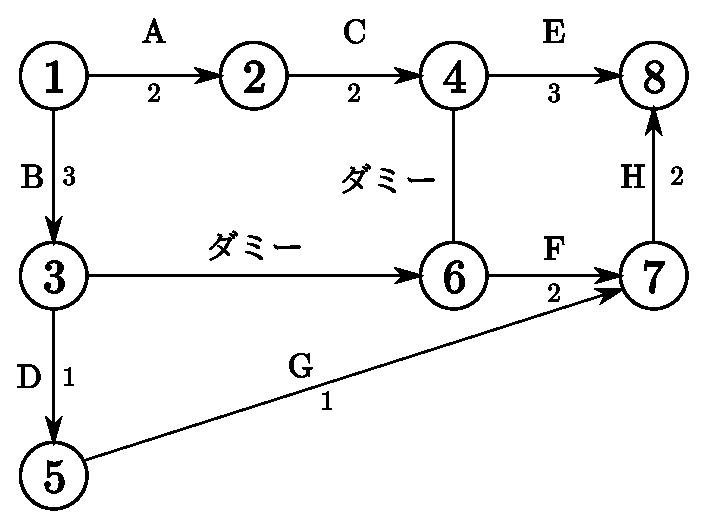
\includegraphics[clip,width=6cm]{fig/eps/arrow.eps}
  \end{center}
  \caption{アローダイアグラム}
  \label{fig:アローダイアグラム}
\end{figure}


\subsection{課題2}
全ての頂点について最早結合点時刻の計算結果を示す.
\begin{table}[!h]
 \begin{center}
  \begin{tabular}{lll}
    $t_1^E = 0$ & $t_2^E = 0+2 = 2$ & $t_3^E = 0+3 = 3$ \\
    $t_4^E = 2+2 = 4$ & $t_5^E = 3+1 = 4$ & $t_6^E = \max(3,\ 4) = 4$ \\
    $t_7^E = \max(5,\ 6) = 6$ & $t_8^E = \max(7,\ 8) = 8$ &\\
  \end{tabular}
 \end{center}
\end{table}

全ての頂点について最遅結合点時刻の計算結果を示す.
\begin{table}[!h]
 \begin{center}
  \begin{tabular}{lll}
    $t_8^L = 8$ & $t_7^L = 8-2 = 6$ & $t_6^L = 6-2 = 4$ \\
    $t_5^L = 6-1 = 5$ & $t_4^L = \min(5,\ 4) = 4$ & $t_3^L = \min(4,\ 4) = 4$ \\
    $t_2^L = 4-2 = 2$ & $t_1^L = \min(0,\ 1) = 8$ &\\
  \end{tabular}
 \end{center}
\end{table}

プログラムによる実行結果のスクリーンショットは課題3の結果と合わせて示す.

\subsection{課題3}
最早$=$最遅結合点時刻となる作業系列を求めると$t_0^E = t_0^L$,$t_2^E = t_2^L$,$t_4^E = t_4^L$,$t_6^E = t_6^L$,$t_7^E = t_7^L$,$t_8^E = t_8^L$となり,$1\rightarrow 2\rightarrow 4\rightarrow 6 \rightarrow 7\rightarrow 8$である.
またFig.~\ref{fig:アローダイアグラム}より作業名で表すと$A\rightarrow C\rightarrow F\rightarrow H$である.

\subsection{結果}
Fig.~\ref{fig:結果のスクリーンショット}にプログラムを実行した結果を示す.

\begin{figure}[!ht]
  \begin{center}
    \includegraphics[clip,width=14cm]{fig/png/result.png}
  \end{center}
  \caption{結果のスクリーンショット}
  \label{fig:結果のスクリーンショット}
\end{figure}

\end{document}